\section{Chemical and Physical Characterization of Precursors}
\label{sec:chemical_and_physical_characterization_of_precursors}

\subsection{Chemical Composition of Precursors}
\label{sec:chemical_composition_of_precursors}

The chemical composition of the aluminosilicate precursors plays a fundamental role in determining their reactivity and suitability for activation in a low-calcium system. 
In this work, the metakaolin (MK) and active silica (SA) precursors were analysed for their oxide content (normalized with respect to the powder fraction) and loss on ignition (LOI), which was found to be 0.69\% and 2.27\%, respectively.
% The results are presented in Table \ref{tab:mk_sa_composition}.

\begin{table}[H]
    \centering
    \caption{Chemical composition (wt \%) of the precursors: metakaolin (MK) and active silica (SA).}
    \label{tab:mk_sa_composition}
    \begin{tabular}{l c c c c}
        \hline
        \multicolumn{1}{c}{Oxide} & \multicolumn{2}{c}{Metakaolin} & \multicolumn{2}{c}{Active Silica} \\
        \cline{2-5}
        & wt (\%) & wt with LOI (\%) & wt (\%) & wt with LOI (\%) \\
        \hline
        K\textsubscript{2}O & 0.21 & 0.20 & 0.74 & 0.73 \\
        CaO & 0.19  & 0.19 & 0.13 & 0.13 \\
        MgO & 2.60 & 2.59 & 0.00 & 0.00 \\
        P\textsubscript{2}O\textsubscript{5} & 0.00 & 0.00 & 0.00 & 0.00 \\
        Cl & 0.00 & 0.00 & 0.12 & 0.12 \\
        SO\textsubscript{3} & 0.00 & 0.00 & 0.15 & 0.15 \\
        SiO\textsubscript{2} & 49.37 & 49.03 & 96.90 & 94.70 \\
        Fe\textsubscript{2}O\textsubscript{3} & 0.77 & 0.76 & 1.78 & 1.74 \\
        Al\textsubscript{2}O\textsubscript{3} & 46.38 & 46.06 & 0.00 & 0.00 \\
        Na\textsubscript{2}O & 0.00 & 0.00 & 0.17 & 0.17 \\
        TiO\textsubscript{2} & 0.49 & 0.48 & 0.00 & 0.00 \\
        \hline
    \end{tabular}
\end{table}

From Table 4.1.1 it is clear that the MK precursor is rich in alumina and contains a significant silica fraction , while the SA is extremely high in silica and essentially alumina-free.
Critically, both materials present very low CaO contents.
The minimal presence of calcium oxide is an important indicator of the low-calcium nature of the precursors, which is a pre-requisite for favoring the formation of potassium aluminosilicate hydrate type gels, rather than calcium-rich gels, as often observed when using ground granulated blast furnace slag \cite{ali2023geopolymer}.


In addition, the low LOI values suggest a limited amount of residual organics or volatile components, which could otherwise interfere with the dissolution kinetics of the aluminosilicates.
Furthermore, the Si/Al molar ratio of MK precursos is approximately 0.9, which will be used with the essentially pure SA to tailor the mix designs for optimal geopolymerization reactions, as presented in Appendix \ref{appendix:mix_designs}.

% Create a slide with this phrase:
In summary, the chemical data confirm that both MK and SA meet the key requirements of (i) high silica and/or alumina content, (ii) low calcium content, and (iii) minimal impurities, thereby validating their use as raw materials for a low calcium alkali-activated binder system.

\subsection{X-Ray Diffraction of Precursors and Alkaline Sources}
\label{sec:x-ray_diffraction_of_precursors_and_alkaline_sources}

XRD analysis was conducted on the precursors and alkaline sources to evaluate phase composition, crystallinity and the presence of amorphous phases. The key observations were as follows:

\begin{table}[H]
    \centering
    \caption{Summary of XRD phase observations for precursors and alkaline sources.}
    \label{tab:precursor_xrd_summary}
    \begin{tabular}{l l}
        \hline
        Material & Key XRD observations \\
        \hline
        MK & Broad amorphous hump near $2\theta \approx 21\degree$, residual quartz peaks (COD 900-9667) \\
        SA & Broad amorphous hump near $2\theta \approx 22.5\degree$, no distinct crystalline phases \\
        Ca(OH)\textsubscript{2} & Crystalline portlandite phase (COD 900-0114) \\
        K\textsubscript{2}CO\textsubscript{3} & Crystalline calcium carbonate phase (COD 900-9644) \\
        \hline
    \end{tabular}
\end{table}

SA and MK both exhibited broad amorphous humps in their XRD patterns, indicative of their largely non-crystalline nature, which is favorable for dissolution during alkali activation.
The MK showed minor crystalline quartz peaks, indicating the presence of impurities, which remains inert during calcination \cite{provis2014geopolymers} and acts as filler without participating in geopolymerization reaction \cite{rakhimova2019metakaolin}.
The alkaline sources displayed sharp diffraction peaks corresponding to their known crystalline phases, confirming their purity.

\section{Microstructural Characterization of Pastes}

\subsection{Scanning Electron Microscopy and Energy Dispersive Spectroscopy}

Scanning electron microscopy of the pastes cured for 3 days revealed a clear dependence of matrix morphology on the Si/Al molar ratio
At Si/Al ratio of 0.9, the SEM images of the paste showed a higher frequency of visibly unreacted precursor particles, together with needle-shaped crystalline features and larger pores. Those unreacted particles are likely some alkali carbonate products that precipitate when mobile alkalis are not fully incorporated into the aluminosilicate gel and subsequently react with atmospheric CO\textsubscript{2} \cite{provis2018alkali}.

By contrast, the Si/Al ratio of 3.0 paste exhibited the densest and most homogeneous matrix, with fewer discernible unreacted particles and a more continuous binder phase.
This indicates that intermediate Si/Al values promote better network polymerization and denser structure.
At Si/Al = 5.0, the SEM images showed residual spherical particles characteristic of silica fume that were not fully reacted after the curing time, indicating that at very high Si/Al the silica supply exceeds the polymerization capacity of the system.

\textcolor{red}{Include SEM images here (three magnifications each) and EDS spectra for Si/Al = 0.9, 3.0, and 5.0}
\textcolor{red}{Three images on each row}
\textcolor{red}{Include stacked bars of K, Al, Si, Ca (At\%) for the three Si/Al ratios }
\textcolor{red}{The remaining information is on Appendix B}


\subsection{X-Ray Diffraction}

X-ray diffraction patterns (3-day curing) of the pastes at different Si/Al ratios showed a persistent amorphous hump in all compositions, indicating the presence of aluminosilicate gel (N-A-S-H).
The hump position and shape were increasingly similar to the active silica (SA) precursor at high Si/Al, consistent with the SEM observation, as it it shifted to the left as silica content increases. 

In agreement with other studies, the geopolymerization process—which is responsible for the strength—is indicated by the presence of the broad hump among $2\theta = 20 \approx 35\degree$.
process shifted the location of the amorphous hump to lower angles as the silica proportion increases \cite{arellano2014geopolymer,lee2017strength, wan2017geopolymerization}.

The patterns of the pastes show sharp peaks of crystalline phases of solid precursors, this indicates that the they were not involved in the geopolymerization process \cite{Geraldo2020}, but were rather present as inactive fillers, as noted by \cite{ruiz2012alkaline}.
The crystalline phases identified in the XRD patterns are presented in Table \ref{tab:xrd_phases_pastes}, showing the semi-quantitative phase composition at 3 days for different Si/Al ratios.

\begin{table}[H]
    \centering
    \caption{Semi-quantitative crystalline phases at 3 days for different Si/Al ratios (XRD).}
    \label{tab:xrd_phases_pastes}
    \begin{tabular}{lrrrrr}
        \hline
        \multicolumn{1}{c}{Phase (\%)} &
        \multicolumn{5}{c}{Si/Al}\\
        \cline{2-6}
        & 0.9 & 2.0 & 3.0 & 4.0 & 5.0 \\
        \hline
        Calcite (CaCO$_3$) & 77 & 56 & 43 & 52 & 79 \\
        Butschliite (K$_2$Ca(CO$_3$)$_2$) & 18 & 29 & 0 & 0 & 0 \\
        Aragonite (CaCO$_3$) & 0 & 0 & 41 & 24 & 0 \\
        Quartz (SiO$_2$) & 6 & 14 & 16 & 17 & 21 \\
        Stishovite (SiO$_2$) & 0 & 0 & 0 & 7 & 0 \\
        \hline
    \end{tabular}
\end{table}

Figure \ref{fig:xrd_pastes} exhibits that at lower Si/Al ratios, the peaks - specially from calcite - are more intense, indicating a higher presence of these crystalline phases from unreacted materials.

% Taken together, the XRD results corroborate the SEM/EDS findings: (i) all mixes formed an amorphous aluminosilicate gel, consistent with low-calcium N-A-S-H-type networks; (ii) Si/Al = 3.0 displayed the microstructurally densest matrix and, correspondingly, lower reliance on alkali-salt precipitation products; (iii) high Si/Al (4–5) retained unreacted silica, evidenced by the hump shape similarity to SA and the SiO₂ fraction; and (iv) low Si/Al (0.9) promoted alkali/carbonate crystallization (including butschliite) consistent with excess free alkali and early carbonation.

\begin{figure}[H]
    \centering
    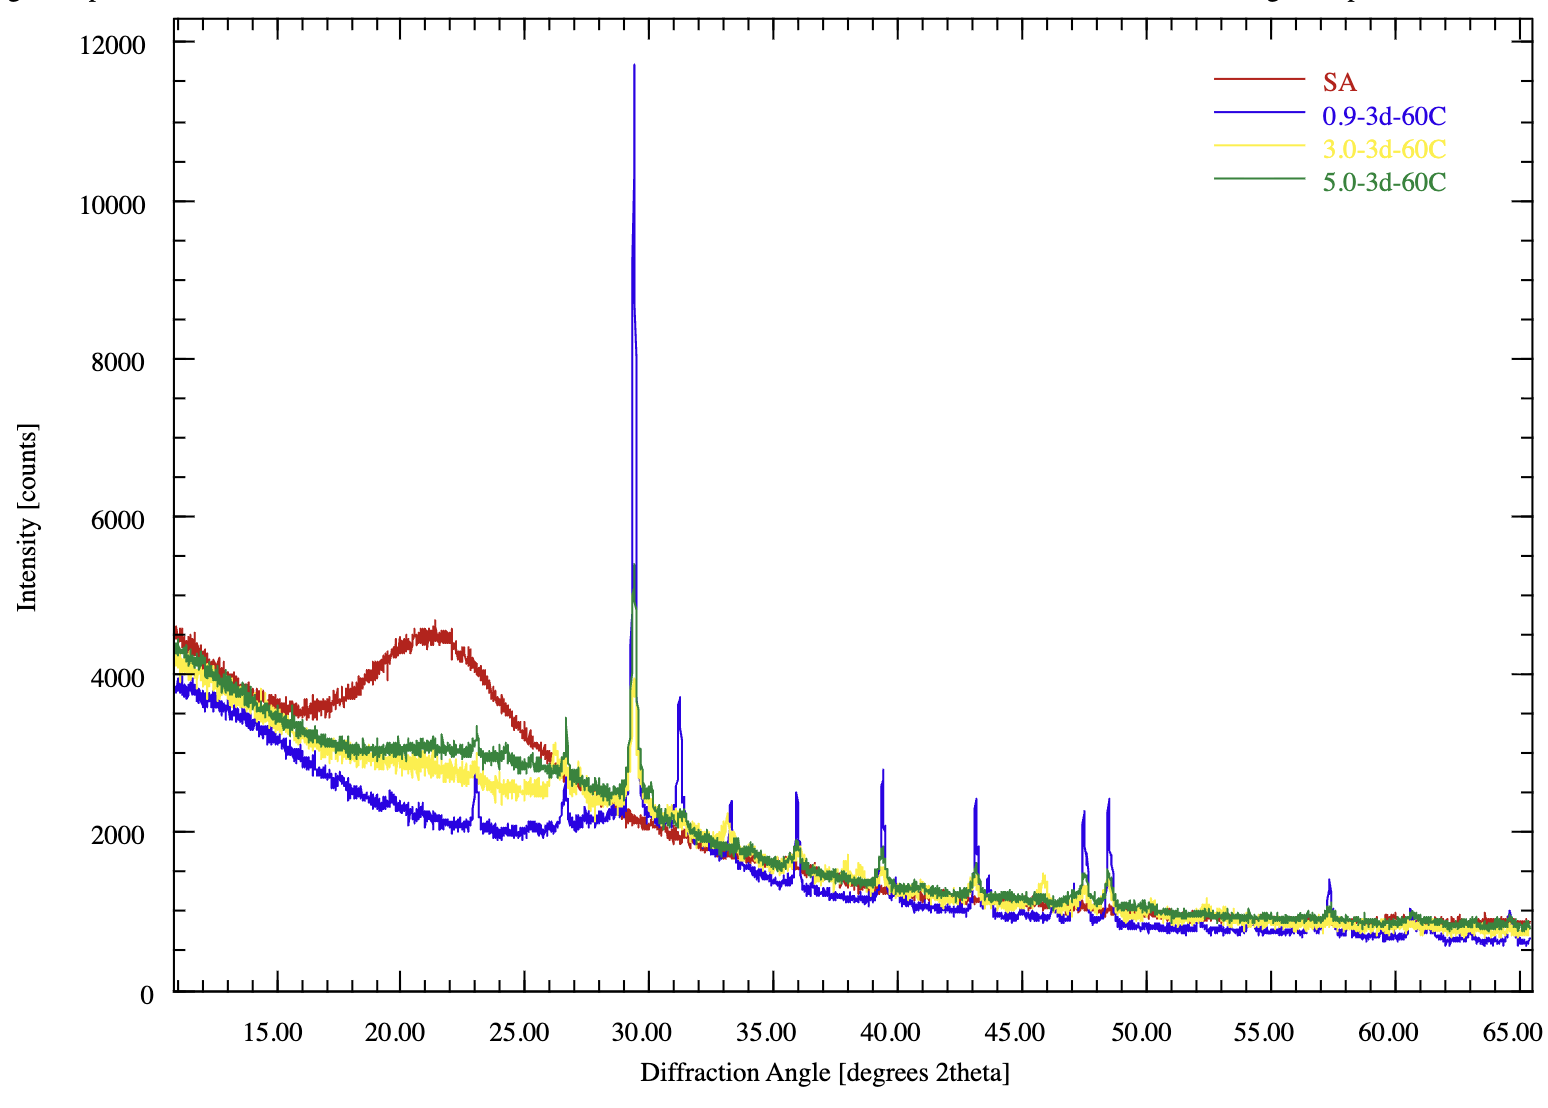
\includegraphics[width=0.8\textwidth]{Cap4/xrd_pastes.png}
    \caption{XRD patterns of pastes at different Si/Al ratios after 3 days of curing.}
    \label{fig:xrd_pastes}
\end{figure}